\section{Introduction}\label{sec:intro}

\paragraph{The question.}
Why is there something rather than nothing, and why this something? We do not answer either half. We ask a narrower
question that can be answered: if existence is taken to be the minimal thing that is not nothing, what does that
minimum force, and what does it leave free? The answer has two halves. Given the chosen form and the inputs of Table~\ref{tab:inputs}, structure follows. The
``which'' is not fixed by it: every number that would single out our world has to be supplied, and no frame on record is
shown to fix one. We locate each of those numbers, and we price each
thing we assume.

\paragraph{The principle.}
We start from one sentence: \emph{existence is what remains when cancelling to nothing cannot complete}. We read it as
a grammar of records.
\begin{itemize}
\item Two integers $(a,b)$ are acted on by two unit moves, $L:(a,b)\mapsto(a,a+b)$ and $R:(a,b)\mapsto(a+b,b)$, and
  by their pull-backs $L^{-1}$ and $R^{-1}$.
\item The non-cancellation is a commutator. The two two-step words $LR$ and $RL$ generate the commutator subgroup of
  $\SL(2,\Z)$, the fundamental group of a once-punctured torus. Their commutator, the two steps followed by their two
  pull-backs, does not return to the start: its trace is $-2$, and the attempt to cancel lands on the puncture, with a
  sign (Proposition~\ref{prop:sign}).
\item A primitive hyperbolic closed path of the moves is a \emph{thread}: a conjugacy class of $\SL(2,\Z)$, a closed geodesic on
  the modular surface. The first such path that mixes the records is $A=LR$, the monodromy of the figure-eight knot's
  complement. Under four stated inputs it is unique (Theorem~\ref{thm:seed}).
\end{itemize}
We do not study one thread. We study all of them at once, the joint action of the moves on the records, which we call
the \emph{weave}. Every result below is a statement about the weave, or is marked as a statement about one thread.

\paragraph{What is forced, and what holds given inputs.}
\begin{enumerate}
\item \textbf{A flavour triplet} (\S\ref{sec:weave}). The moves permute the records' three non-zero parities as
  $S_3$, on every thread. The odd-trace threads receive the binary tetrahedral group $2T$ at the threads' common
  point, acting irreducibly on the three parity lines: proved for every odd-trace word. The arithmetic of that point (a prime above $3$) is a census law to length eight.
\item \textbf{The triplet is modular} (\S\ref{sec:modular}). A stated lift of the moves to the triplet is the multiplier of
  $\eta^{21}(\theta_2^2,\theta_3^2,\theta_4^2)$: the weight-one theta triplet of $\Gamma(4)$, the triplet of modular
  flavour models~\cite{NovichkovPenedoPetcov2021}, twisted by a character of $\eta$ and up to a monomial intertwiner.
  The classical part is that the modular group permutes the three even theta characteristics; a power of the eta
  character is automatic once the lift agrees with the theta multiplier projectively. What is computed is that
  agreement, the exponent $21$ and the hand.
\item \textbf{A null vector of the coupling ansatz in the fibre frame} (\S\ref{sec:couplings}). On the fibre, given the triplet
  postulate, the zero modes' pairing triplet is isotropic at every point (Jacobi's
  $\theta_3^4=\theta_2^4+\theta_4^4$), so every single-point coupling has a two-sided null vector. The statement is
  frame-dependent, and we say where it fails. For a real direction the ratio of the other two singular values is at least $\tfrac12$; a hierarchy needs a complex direction near the isotropic cone (Theorem~\ref{thm:isotropy}).
\item \textbf{The coupling's determinant factors through two defects} (Theorem~\ref{thm:joint}). In the twisted frame the coupling's
  determinant and adjugate factor exactly:
  \[
    \det Y = 4\det S\,\det M\,\tr(\epsilon S M^{T}),\qquad
    \adj Y = \det S\,A(M)+\det M\,P\,A(S).
  \]
  Read through the dictionary of Table~\ref{tab:inputs}, the product of the masses factors through the two defects and their
  pairing, and the squared masses are the roots of a cubic whose other two coefficients are norms of the coupling.
\item \textbf{A conditional index} (\S\ref{sec:three}). With the triplet postulate, one unit at the cusp and an extreme
  boundary domain, on $M_{1,2}$ read as the weave's surface and with an index formula taken from the record, the
  four-dimensional index is $\pm3$. The $3$ is the postulated triplet's dimension. Under $2T$ alone a domain respecting
  the symmetry allows $\pm1$ as well; with the parity grading only $\pm3$ is kept.
\item \textbf{The moves' anomaly and the strong angle} (\S\ref{sec:anomaly}). The triplet's determinant character is
  $\chi_\eta^9$. If the moves act on the Standard Model's fermions as a symmetry, their mixed anomaly with QCD vanishes
  at the level of the character exactly when they act on left- and right-handed quarks alike; with $\mathrm{SU}(2)$ it
  never vanishes. On the ruled branch's ansatz, a counterterm in $\arg\eta(\tau)$ cancels the anomaly when the coupling
  weights satisfy a congruence. With it, the strong angle is constant at weight one, and at weights two and three, with real
  coefficients, it differs from its constant term by a multiple of $\pi$ only where CP is conserved. The constant term
  is free, so the strong angle, one of the nineteen, is not fixed. These are conditions of consistency, not identifications.
\end{enumerate}

\begin{figure}[t]
\centering
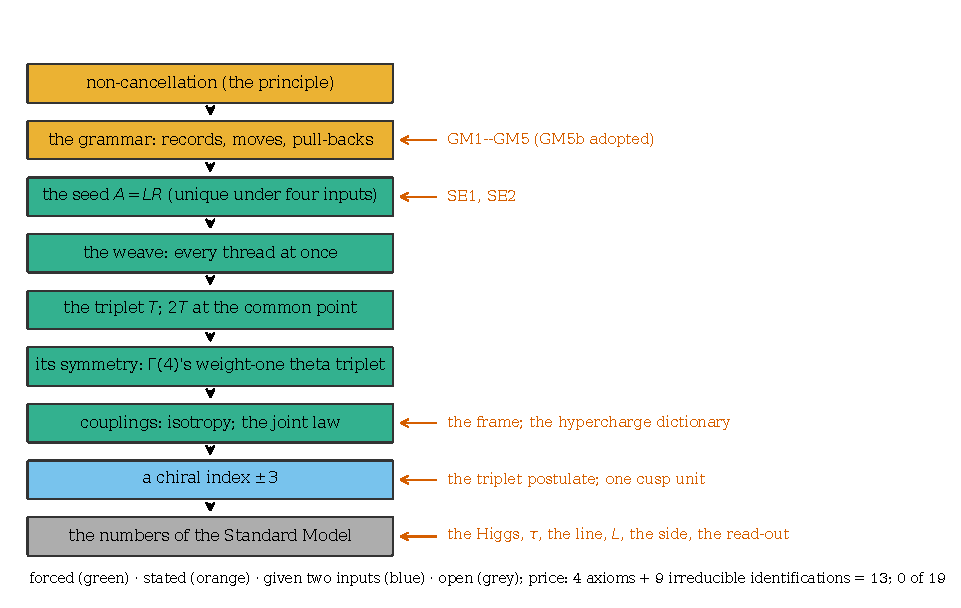
\includegraphics[width=0.92\linewidth]{figures/fig_chain}
\caption{The chain and its prices: what follows from the stated inputs of its section (green), what is stated (orange), what
also needs tagged postulates (blue), and what is open (grey). Inputs enter from the right. The seed is a side branch of
the grammar. A drawn schematic of Table~\ref{tab:inputs}.}\label{fig:chain}
\end{figure}

\paragraph{What is not.}
In the frames we studied, the same structure fixes none of the Standard Model's thirteen flavour numbers (\S\ref{sec:boundary}). The boundary
is as sharp as the forced half:
\begin{itemize}
\item in the frames where the inner automorphisms act, every residual subgroup of the weave's group either degenerates
  the masses or leaves them free, and none that reduces the count of mixing parameters is compatible with the CKM data
  at $3\sigma$;
\item no frame on record is shown to satisfy all of the principle's demands;
\item on the ruled branch the triplet's parameter-free coupling has $m_2/m_1\ge\tfrac12$ at every modulus
  (Corollary~\ref{cor:halffloor}), so it carries no hierarchy anywhere;
\item a sealed census finds that one Higgs at the symmetric point $\tau=\omega$ reproduces the five non-electron mass
  ratios on none of the admissible lines. The miss is the down--lepton ratio $(m_\mu/m_\tau)/(m_s/m_b)$, which the
  data put at $3.14$ (from $2.9$ to $3.4$ within the strange-quark mass's uncertainty alone);
\item whatever chooses the numbers is not given by the symmetry alone, although it acts at a symmetric point.
\end{itemize}

\paragraph{The motion.}
The grammar's states move. A random walk of steps and pull-backs escapes at a positive rate: for equal weights by the
theorems of Kesten and Furstenberg, and at the other weights by Furstenberg's theorem, since the support generates
$\SL(2,\Z)$; the values are measured. Two sealed arcs read that motion: B1663, and B1666, a scoreboard computed after
the gates of B1664 and B1665 had failed and their read-outs had been seen.
\begin{itemize}
\item The pull-back's strength sets the probability of the side the end lies on (from $1.000$ to $0.531$) and the speed, but not
  the defect it averages, to the test's resolution (B1663).
\item Averaged trace by trace, the threads approach the modular surface's constant mode ($0.3144$ at the largest
  traces against $0.31500491$, the gap shrinking as $t^{-0.51\pm0.05}$, a read-out): the weave side of the trace formula comes out where
  the wave side says, as equidistribution requires (a check of the instrument).
\item The amplitude built from the matter's defect returns after one period by the multiplier of $\eta^6$ (Theorem~\ref{thm:phase}). The normalised coherence of the cusp family $L^{4m+1}R$ climbs
  toward one, and the root $LR$ is not singled out (a read-out; the size of the coherent amplitude is not compared).
\end{itemize}
These are statements about the mathematics of the motion. We do not claim the motion is physical.

\paragraph{The record.}
The computations are archived in a public repository~\cite{OriginAxiomRepo}. A label such as B1659 names one
computation there (an \emph{arc}), with its preregistration, instrument, output and \emph{lock}, a test in the
repository's suite that fails if the result changes. A \emph{scoreboard} is a result computed on data that were already
seen, and is called so. A \emph{tagged} input is a working postulate whose results carry the word ``given''. The
program's work runs on several parallel lines on the same record; their cross-checks are internal to the program, not
external review.

\paragraph{The price.}
Every input is stated in Table~\ref{tab:inputs}, with what it buys and what would discharge it: the principle, the
grammar and the root's two conditions, one adopted reading, the choices (positivity, orientation, the boundary domain, the
frame, the modulus and the lines, the canonical horocycle, the hand and the $\eta$ twist, the Higgs's type and locus), the
tagged postulates, the readings (the weave's surface, the modular-flavour ansatz, the index formula), and the
identifications that turn structure into physics. No value of the Standard Model is derived:
none of its nineteen parameters. We built the computations as sealed tests: each preregistered,
run once per sealed version, and its output committed before it was read. The paper keeps its failures, including two failed gates of our own (\S\ref{sec:methods}).

\reading{The principle asks for something that cannot cancel. The grammar's answer is a motion: steps and their
pull-backs that never settle. The structure that motion carries holds on the stated inputs. What it leaves free is the choice of a
world.}
